\documentclass[10pt,a4paper]{article}
\usepackage[utf8]{inputenc}
\usepackage[english]{babel}
\usepackage[square, numbers, sort&compress]{natbib}
\usepackage{graphicx}
\usepackage{float}
\usepackage{amsmath}
\usepackage{amsfonts}
\usepackage{amssymb}
\usepackage{media9}
\usepackage{epstopdf}
\usepackage{color}
\usepackage{fancyhdr}
\usepackage{lastpage}	
\usepackage{parskip}
\usepackage[scaled]{helvet}
\usepackage{blindtext}
\usepackage{sectsty}
\usepackage{multicol}
\usepackage{enumitem}
%\usepackage[svgnames]{xcolor}
\usepackage[labelfont={color=LibrelloColor,bf}, labelsep=period]{caption}
\renewcommand*{\familydefault}{\sfdefault}
\usepackage[left=1.75cm,right=1.75cm,top=1.75cm,bottom=3.75cm]{geometry}
\usepackage{titlesec}
\usepackage{svg}
\usepackage{flushend}
\PassOptionsToPackage{normalem}{ulem}
\usepackage{ulem}
	\providecolor{added}{rgb}{0,0,1}
	\providecolor{deleted}{rgb}{1,0,0}
	%% Change tracking with ulem
	\newcommand{\added}[1]{{\color{added}{}#1}}
	\newcommand{\deleted}[1]{{\color{deleted}\sout{#1}}}
\usepackage{setspace}
\usepackage[hyphens]{url}

% Green - CiS, OF
\definecolor{LibrelloColor}{RGB}{0,85,0}
% Red - JoHS
%\definecolor{LibrelloColor}{RGB}{128,0,0}


\usepackage[hidelinks, urlcolor=LibrelloColor]{hyperref}
\urlstyle{same}
\raggedcolumns
\flushcolumns
\usepackage{etoolbox}
\usepackage{caption}
\usepackage{supertabular}
\usepackage{booktabs}
\usepackage{microtype}
\usepackage{threeparttable}
\usepackage{doi}
\usepackage{balance}
\usepackage{enumitem}
\usepackage{eurosym}

\usepackage[color=yellow,icon=Comment,hoffset=-10mm, author=Librello Editorial's Office]{pdfcomment}

\titleformat{\section}
{\color{LibrelloColor}\normalfont\bfseries\filright}
{\color{LibrelloColor}\thesection.}{0.5em}{}

\titleformat{\subsection}
{\color{LibrelloColor}\normalfont\itshape\filright}
{\color{LibrelloColor}\thesubsection.}{0.5em}{}

\titleformat{\subsubsection}
{\color{LibrelloColor}\normalfont\itshape\filright}
{\color{LibrelloColor}\thesubsubsection.}{0.5em}{}

\usepackage{array} %criando coluna de largura fixa alinhada a esquerda
\newcolumntype{L}[1]{>{\raggedright\let\newline\\\arraybackslash\hspace{0pt}}p{#1}}
%criando coluna de largura fixa alinhada a direita
\newcolumntype{R}[1]{>{\raggedleft\let\newline\\\arraybackslash\hspace{0pt}}p{#1}}
\renewcommand{\arraystretch}{1.3}
\titlespacing\section{0pt}{12pt}{12pt}
\titlespacing\subsection{0pt}{12pt}{12pt}
\titlespacing\subsection{0pt}{12pt}{12pt}	
\renewcommand*{\refname}{References and Notes}

\fancypagestyle{document}{
	\renewcommand{\footrulewidth}{0pt}
	\renewcommand{\headrulewidth}{0pt}
	\renewcommand{\footrulewidth}{0pt}
	\renewcommand{\headrulewidth}{0pt}
	\renewcommand{\footskip}{40pt}
	\cfoot{\normalfont\thepage}
	\rhead{}\lhead{}
}

\fancypagestyle{firstpage}{
	\renewcommand{\footrulewidth}{0pt}
	\renewcommand{\headrulewidth}{0pt}
	\renewcommand{\footrulewidth}{0pt}
	\renewcommand{\headrulewidth}{0pt}
	\renewcommand{\footskip}{70pt}
	%CiS
	\lhead{Challenges in Sustainability $\mid$ 2017 $\mid$ Volume 5 $\mid$ Issue 1 $\mid$ Pages \thepage--\pageref{LastPage} \\DOI: 10.12924/cis2017.05010024\\
	ISSN: 2297--6477}
	\rhead{\includegraphics[height=0.59in]{CiS.eps}}
	%JoHS
%	\lhead{Journal of Human Security $\mid$ 2016 $\mid$ Volume 12 $\mid$ Issue 1 $\mid$ Pages \thepage--\pageref{LastPage} \\DOI: 10.12924/johs2016.12010112\\
%	ISSN: 1835--3800}
%	\rhead{\includegraphics[height=0.59in]{JoHS.eps}}
	%OF
%	\lhead{Organic Farming $\mid$ 2016 $\mid$ Volume 2 $\mid$ Issue 1 $\mid$ Pages \thepage--\pageref{LastPage} \\DOI: 10.12924/of2016.02010023\\
%	ISSN: 2297--6485}
%	\rhead{\includegraphics[height=0.59in]{OF.eps}}	
	\lfoot{\footnotesize © 2017 by the authors; licensee Librello, Switzerland. This open access article was published\\ under a Creative Commons Attribution License (\url{http://creativecommons.org/licenses/by/4.0/}).}
	\cfoot{}
	\rfoot{\vspace*{-24pt}\includegraphics[height=0.49in]{librello.eps}}

}

\makeatletter
\def\NAT@def@citea{\def\@citea{\NAT@separator}}
\makeatother

\begin{document}
\flushcolumns
\raggedcolumns

\pagestyle{document}
\thispagestyle{firstpage}

\vspace*{70pt}

\setlength{\parindent}{0cm}
%\textit{Research Article}
%\textit{Review}
\textit{Opinion}
\vspace*{-12pt}

\begin{center}
\line(1,0){500}
\end{center}

\vspace*{12pt}
\begin{flushleft}
\begin{LARGE}
\textbf{{\color{LibrelloColor} Making Research Matter More---Working with Action Research and Film in Sustainability Science}}\\
\end{LARGE}

\vspace*{12pt}

Elina Andersson* and Ann Åkerman

\vspace*{6pt}

Lund University Centre for Sustainability Studies (LUCSUS),  Lund, Sweden

\vspace*{6pt}

* Corresponding author: E-Mail:elina.andersson@lucsus.lu.se; Tel.: +46 462228416
%
%\vspace*{6pt}

%Submitted: 20 March 2016 $\mid$ In revised form: 21 July 2016 $\mid$ Accepted: 12 October 2016 $\mid$\\
Published: 1 March 2017
\end{flushleft}
\setcounter{page}{24}


\vspace*{-18pt}
\begin{center}
\line(1,0){500}
\end{center}

\vspace*{12pt}
%\vspace{\baselineskip}

\begingroup\leftskip= 1cm\rightskip 1cm  

%\textbf{{\color{LibrelloColor}Abstract:}} Policies of the European Union cover a range of social, environmental and economic aspirations and the current environmental directives and laws have evolved from a suite of norms which have changed over time.  These may be characterised loosely according to `Three Ps': Practical, those taking an anthropocentric approach; Pure, those taking an ecocentric approach and Popular, those appealing to the general public. In this paper I use these three perspectives as a tool to analyse the complexity and identify contradictions in European aquatic environmental legislation. Some trade-offs between development and conservation are identified and used to characterise the potential qualities of more successful agency to achieve environmental goals in the governance of European aquatic environments.

%\textbf{{\color{LibrelloColor}Keywords:}} biodiversity; environmental policy; ecosystem services; transformation
\par\endgroup
 
\setlength{\parindent}{0.5cm}
\setlength{\parskip}{0cm}
\setlength{\bibsep}{0cm}

\vspace*{5mm}
%\vspace*{20mm}

\begin{multicols}{2}

\noindent Advocacy for both critical analysis of social and environmental change and a more solutions-oriented agenda has been a central mission of sustainability science since its inception \citep{r08}. To this end, integration of knowledge across disciplinary divides and inclusion of non-academic actors into the research process have been widely promoted (e.g. \citep{r01, r02, r03}). Aspirations to link knowledge to action do not only bear on processes of knowledge generation, but also on strategies for research outreach.

The short film presented here---``Making research matter---From knowledge to action with farmers in Uganda''' (Video \ref{video})---builds on a PhD project in sustainability science \citep{r04} and is part of research outreach efforts at Lund University Centre for Sustainability Studies. It represents one attempt to explore and pursue the use of film as an alternative medium tool for research communication. At the same time, this film presents a concrete example of how action-oriented research can be employed in sustainability science to generate place-based knowledge as well as practical outcomes in favour of sustainability. More specifically, the film focuses on land degradation---a serious sustainability challenge in many parts of the world---and reflects a process in which smallholder farmers in Uganda were involved in research to jointly define problems and develop a partial solution to soil fertility problems, namely the use of human urine as fertilizer in food production.

\textls[13]{The film provides insights into persistent problems of food insecurity and low agricultural production experienced by a smallholder community in eastern Uganda. The situation in the region reflects the generally dire conditions experienced in many parts of rural sub-Saharan Africa, which indeed is one of the ``grand challenges'' for sustainability science \citep{r05}. The film shows how farmers' everyday lives are affected by land degradation, in terms of nutrient depletion and erosion, and how their ability to produce enough food is seriously hampered by multiple and interlocking challenges, including environmental change, socio-economic vulnerability and rural marginalization. The film focuses not only on these challenges, but also illuminates people's agency and creativity in the way they cope with and tackle problems, with an emphasis on farmers' collective strategies in the form of self-organized community groups. Through pooling of resources, exchange of knowledge and joint experimentation, such groups serve as arenas for `everyday politics' \citep{r06}, and the creation of strategies to expand the room for manoeuvre in struggles over resources while seeking alternative development pathways. Building on farmers' existing collective action, the film, furthermore, describes the initiation of a collaborative experimentation process in which urine fertilizer was tested, positively evaluated and eventually disseminated through various strategies. The process is an example of how transdisciplinary research can guide sustainability pathways through locally-anchored knowledge, taking into account environmental and technological---as well as social dimensions.}

\end{multicols}

\renewcommand{\figurename}{Video}

\noindent
\begin{minipage}{\columnwidth}
\centering
\resizebox{0.9\columnwidth}{!}
{\includemedia[
  width=1\linewidth,height=0.6\linewidth,
  activate=pageopen,
  flashvars={
    modestbranding=1 % no YT logo in control bar
   &autohide=1       % controlbar autohide
   &showinfo=0       % no title and other info before start
  }
]{}{https://www.youtube.com/v/9jc3HJ1Y4nk?rel=0}}
\captionof{figure}{Making research matter more---From knowledge to action with farmers in Uganda. The video is also available at \url{https://www.youtube.com/v/9jc3HJ1Y4nk?rel=0}. \label{video}}
\vspace{\baselineskip}
\end{minipage}

\begin{multicols}{2}

Rather than portraying farmers as passive victims of environmental change, the film emphasizes local agency in response to change. It also demonstrates how processes of collaborative inquiry can cultivate a sense of pride and solution ownership among the participants. As one farmer expressed: ``There is science now even in agriculture!'' \citep{r04}. From a social learning perspective, it demonstrates that the process of inquiry is equally as important as the practical outcomes, stimulating critical reflection on problems among farmers and inspiring them to continue with experimentation. This illustrates how transdisciplinarity, in the context of sustainability science, can be ``both a tool and a project'' \citep{r07}.

\textls[-30]{With this film we want to encourage additional efforts to pursue socially-engaged research on issues of pressing concern to people and tangibly contribute to strategies and action towards sustainability. Taking research outreach efforts seriously also reflects the ambitions of transdisciplinary research to concretely bridge science and society. The medium of film offers the potential for broad outreach and effective communication with a diversity of actors, including those who lack access to traditional forms of academic publishing. The film, therefore, is also an example of moving beyond the mere ``reporting back'' of findings to those directly involved in the research. To further enhance the practical use of the research findings, we have also produced a short instruction film on the use of urine as fertilizer, serving as a practical tool to disseminate knowledge about, and encourage uptake of, the practice. While publishing scientific articles will continue to be the most common method of research communication, and there are still numerous challenges associated with film as an effective form of research dissemination \citep{r09}, it is positive and promising that the medium of film is increasingly welcome into the realm of academic publishing.   }

%\section*{Acknowledgements}

\end{multicols}

\vspace{\baselineskip}

\begin{multicols}{2}
\renewcommand*{\refname}{\normalsize{References and Notes}}

\begin{footnotesize}
\bibliographystyle{vancouver_Librello}
\bibliography{309-Biblio}



\end{footnotesize}

\end{multicols}

\end{document}







\vspace{\baselineskip}

\noindent
\begin{minipage}{\columnwidth}
\centering
\resizebox{\columnwidth}{!}
{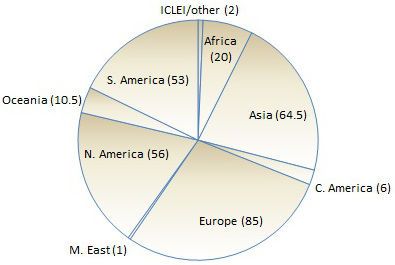
\includegraphics[width=\textwidth]{Fig01.jpg}}
\captionof{figure}{Community gardens in the north of Lisbon (Portugal). \label{Fig01}}
\end{minipage}




\end{multicols}
\vspace{\baselineskip}

\setlength{\tabcolsep}{3pt}
\noindent
\begin{footnotesize}
\begin{minipage}{\columnwidth}\centering
\captionof{table}{Results of a General Linear Model for the proportion of agricultural land under organic farming in French Departments (2008) as a function of plant biodiversity, landscape connectivity, proportion of Natura 2000 protected areas, latitude, longitude, altitude, human population size and department area. The number of data points is 95, the adjusted R$^2$ of the model 0.50, and the intercept 1.457 (s.e. = 2.074).}
\label{Tab01}
\begin{tabular}{lrrrrrrrr}
\toprule
 & N of plant taxa & Landscape connectivity & \% Natura 2000 & Latitude & Longitude & Altitude & Human population & Area \\
\midrule
parameter estimate & 0.264 & 0.047 & 0.113 & -0.084 & 0.003 & 0.038 & 0.056 & 0.327 \\
s.e. & 0.486 & 0.101 & 0.09 & 0.024 & 0.017 & 0.172 & 0.132 & 0.139 \\
\textit{P}-value & 0.59 & 0.64 & 0.21 &\textbf{ \textless0.001} & 0.87 & 0.82 & 0.67 & \textbf{0.02}\\
\bottomrule
\end{tabular}
\end{minipage}

\end{footnotesize}

\vspace{\baselineskip}
\begin{multicols}{2}


\begin{enumerate}[label=\alph*)]
\item
\end{enumerate}